\subsection{Iteration for Solving $x = g(x)$}

\frame{
\begin{block}{Iteration}
As the name suggests, a process is repeated until an answer is achieved.
\end{block}
\begin{itemize}
\item A rule of function $g(x)$
\item Starting value $p_0$
\item a sequence of values $\left\{ p_k \right\}$ is obtained using the iterative rule $p_{k+1} = g( p_k )$. 
\end{itemize}
\begin{block}{The sequence has the pattern}
\begin{table}[!h]
\begin{tabular}{l l l}
$p_0$ & & (starting value) \\
$p_1$ & = $g(p_0)$ & \\
$p_2$ & = $g(p_1)$ & \\
& $\vdots$ & \\
$p_k$ & = $g(p_{k-1})$ & \\
$p_{k+1}$ & = $g(p_k)$ & \\
& $\vdots$ & 
\end{tabular}
\end{table}
\end{block}
}

\frame{
\begin{block}{Example.}	
The iterative rule $p_0 = 1$ and $p_{k+1} = 1.001 p_k$ for $k = 0, 1, \ldots$ produces a divergent sequence. 
\end{block}
The first $100$ terms look as follows:
\begin{equation*}
\begin{array}{l l l l}
p_1 & =1.001p_0 & = (1.001)(1.000000) & = 1.001000, \\ 
p_2 & =1.001p_1 & = (1.001)(1.001000) & = 1.002001, \\
p_3 & =1.001p_2 & = (1.001)(1.002001) & = 1.003003, \\
\vdots & & \vdots & \vdots	\\ 
p_{100} & = 1.001 p_{99} & = (1.001)(1.104012) & = 1.105116.
\end{array}
\end{equation*}
The process can be continued indefinitely, and it is easily shown that $\lim_{n \rightarrow \infty} p_n = +\infty$.
}

\frame{
\begin{block}{Problems need to solve!}
\begin{itemize}
\item {\Large What can we learn from an unending sequence of numbers? }
\vspace{0.5cm}
\item {\Large If the numbers tend to a limit, we feel that something has been achieved. But what if the numbers diverge(发散) or are periodic(周期的)? }
\end{itemize}
\end{block}
}


\frame{
\frametitle{Finding Fixed Points}
\begin{block}{Definition .}
A {\Large fixed point} of a function $g(x)$ is a real number $P$ such that $P =g(P)$.\\
Geometrically, the fixed points of a function $y = g(x)$ are the points of intersection of $y = g(x)$ and $y = x$.
\end{block}
\vspace{0.5cm}
\begin{block}{Definition .}
The iteration $p_{n+1} = g(p_n)$ for $n = 0, 1, \ldots $ is called {\Large fixed-point iteration}.
\end{block}
}

\frame{
\begin{block}{Theorem .}
Assume that $g$ is a {\Large continuous function} and that $\{p_n\}_{n=0}^{\infty}$ is a sequence generated by fixed-point iteration.  \\
\vspace{0.5cm}
if $\lim_{n \rightarrow \infty} p_n = P$, then $P$ is a fixed point of $g(x)$.
\end{block}
\begin{block}{Proof.}	
If $lim_{n \rightarrow \infty} p_n = P$, then $lim_{n \rightarrow \infty} p_{n+1} = P$. It follows from this result, the
continuity of $g$, and the relation $p_{n+1} = g ( p_n )$ that
\begin{equation*}
g(P) = g \left( \lim_{n \rightarrow \infty} p_n \right) = \lim_{n \rightarrow \infty}  g(p_n)= \lim_{n \rightarrow \infty} p_{n+1} = P.
\end{equation*}
Therefore, $P$ is a {\Large fixed point} of $g(x)$.
\end{block}
}

\frame{
\frametitle{Example .}
\begin{block}{}
Consider the convergent iteration  \\
$p_0 =0.5$ and $p_{k+1} =e^{-p_k}$ for $k = 0, 1, \ldots$
\end{block}
\pause
The first $10$ terms are obtained by the calculations
\begin{table}[!h]
\begin{tabular}{l}
$p_1 = e^{-0.500000} = 0.606531$\\
$p_2 = e^{-0.606531} = 0.545239$ \\
$p_3 = e^{-0.545239} = 0.579703$\\
$\vdots$ \\
$p_9 = e^{-0.566409} = 0.567560$ \\
$p_{10} = e^{-0.567560} = 0.566907$ \\ 
\end{tabular}
\end{table}
The sequence is {\Large converging}, and further calculations reveal that
\begin{equation*}
lim_{n \rightarrow \infty} p_n = 0.567143....
\end{equation*}
Thus we have found an approximation for the fixed point of the function $y = e^{-x}$ .
}

\frame{
\begin{block}{Theorem.}	
Assume that $g \in C[a, b]$.
\begin{itemize}
\item If the range of the mapping $y = g(x)$ satisfies $y \in [a,b]$ for all $x \in [a,b]$, then $g$ has a fixed point in $[a, b]$.
\item Furthermore, suppose that $g′(x)$ is defined over $(a,b)$ and that apositive constant $K < 1$ exists with $|g′(x)| \le K < 1$ for all $x \in (a,b)$; then $g$ has a unique fixed point $P$ in $[a, b]$.
\end{itemize}
\end{block}
}

\frame{
\frametitle{Proof of Theorem.}
If $g(a) = a$ or $g(b) = b$, the assertion is true.  \\
Otherwise, the values of $g(a)$ and $g(b)$ must satisfy $g(a) \in (a, b]$ and $g(b) \in [a, b)$.  \\
The function $f (x) ≡ x - g(x)$ has the property that
\begin{equation*}
f (a) = a - g(a) < 0
\end{equation*}	
and
\begin{equation*}
f (b) = b - g(b) > 0.
\end{equation*}
Now apply the intermediate value theorem, to $f (x)$, with the constant $L = 0$, and conclude that there exists a number $P$ with $P \in (a,b)$ so that $f(P) = 0$. Therefore, $P = g(P)$ and $P$ is the desired fixed point of $g(x)$.
}

\frame{
\frametitle{Proof of Theorem (continued)}
By way of contradiction, let us make the additional assumption that there exist two fixed points $P_1$ and $P_2$. 
Apply  the mean value theorem, and conclude that there exists a number $d \in (a, b)$ so that
\begin{equation*}
g′(d)= \frac{g(P_2)-g(P_1)}{P2 - P1}. 
\end{equation*}
Use the facts that $g(P_1) = P_1$ and $g(P_2) = P_2$ to simplify the right side of the equation  and obtain
\begin{equation*}
g′(d) = \frac{P_2 - P_1}{P_2 - P_1} = 1. 
\end{equation*}
But this contradicts the hypothesis in above equation that $|g′(x)| < 1$ over $(a,b)$, so it is not possible for two fixed points to exist. Therefore, $g(x)$ has a unique fixed point $P$ in $[a, b]$ under the conditions given in above equation.
}

\frame{
\begin{block}{Theorem  (Fixed-Point Theorem).}
Assume that 
\begin{itemize}
\item (i) $g, g′ \in C[a, b]$, 
\item (ii) $K$ is a positive constant, 
\item (iii) $p_0 \in (a, b)$, 
\item (iv) $g(x) \in [a, b]$ for all $x \in [a, b]$.
\end{itemize}
\vspace{0.5cm}
\begin{itemize}
\item If $|g′(x)| \le K < 1$ for all $x \in [a,b]$, then the iteration $p_n = g(p_{n-1})$ will converge to the unique fixed point $P \in [a, b]$. 
$\rightarrow$
In this case, $P$ is said to be an attractive fixed point.
\item If $|g′(x)| > 1$ for all $x \in [a,b]$, then the iteration $p_n = g(p_{n-1})$ will not converge to $P$ . 
$\rightarrow$
In this case, $P$ is said to be a repelling fixed point and the iteration exhibits local divergence.
\end{itemize}
\end{block}
}

\frame{
\begin{block}{Corollary\footnote{推论} 1.1.}
Assume that $g$ satisfies the hypothesis given in of Theorem 1.3. 
Bounds for the error involved when using pn to approximate $P$ are given by
\begin{equation*}
\left| P-p_n \right| \le K^n \left| P-p_0 \right| \ \ \ for \ all \ n\ge 1 
\end{equation*}
and
\begin{equation*}
\left| P-p_n \right| \le \frac{K^n \left| p_1-p_0 \right|}{1-K} \ \ \ for \ all \ n \ge 1. 
\end{equation*}
\end{block}
}

\frame{
\frametitle{Graphical Interpretation of Fixed-Point Iteration}
\begin{columns}
\begin{column}{0.5\textwidth}
\begin{figure}
\begin{center}
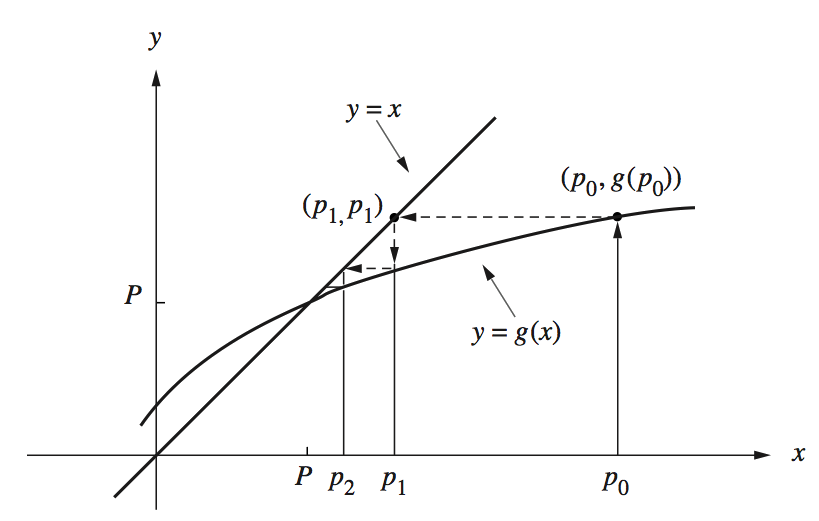
\includegraphics[width=60mm]{chap-1/fig_2-4.png}
\caption{Monotone convergence (单调收敛) when $0 < g`(P) < 1$}
\end{center}
\end{figure}
\end{column}
\begin{column}{0.5\textwidth}
\begin{figure}
\begin{center}
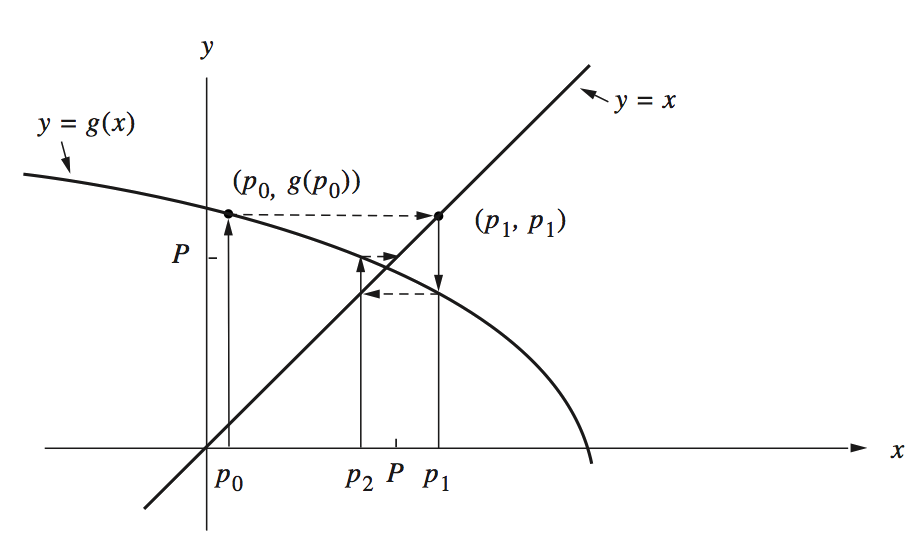
\includegraphics[width=60mm]{chap-1/fig_2-4_2.png}
\caption{Oscillating converagence (振荡收敛) when $-1 < g`(P) < 0$}
\end{center}
\end{figure}
\end{column}
\end{columns}
}

\frame{
\begin{block}{}
if $|g`(P)| > 1$, then the iteration $p_{n+1} = g(p_n)$ produces a sequence that diverages away from $P$.
\end{block}
\begin{columns}
\begin{column}{0.5\textwidth}
\begin{figure}
\begin{center}
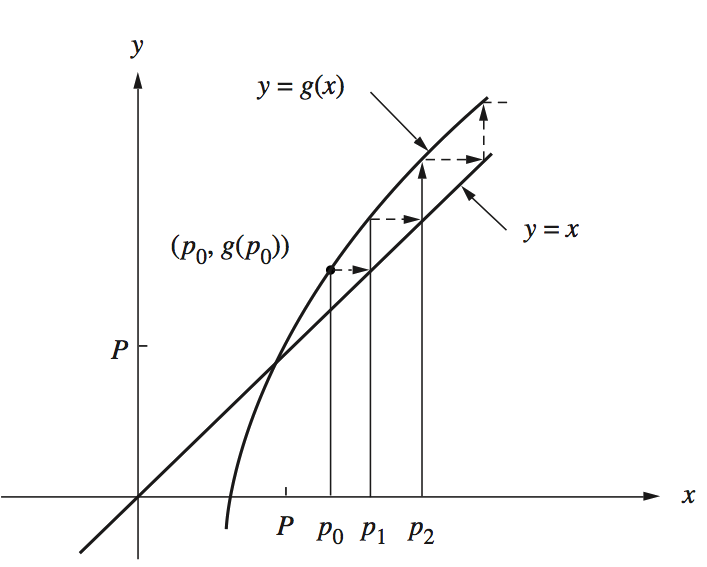
\includegraphics[width=60mm]{chap-1/fig_2-5.png}
\caption{Monotone divergence when $1 < g`(P)$}
\end{center}
\end{figure}
\end{column}
\begin{column}{0.5\textwidth}
\begin{figure}
\begin{center}
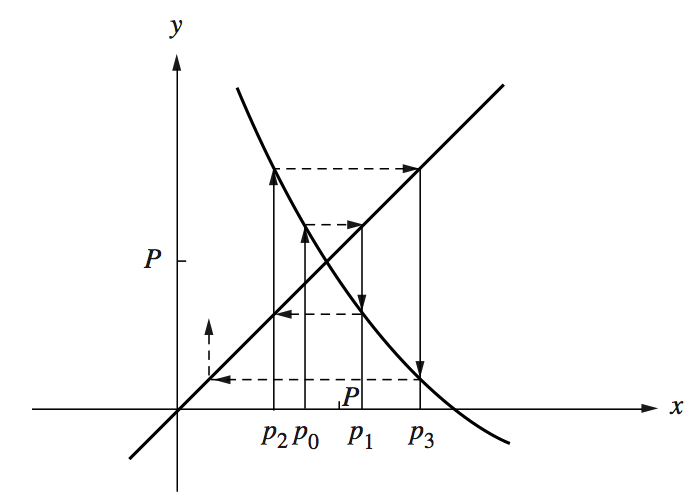
\includegraphics[width=60mm]{chap-1/fig_2-5_2.png}
\caption{Divergent Oscillating when $g`(P) < -1$}
\end{center}
\end{figure}
\end{column}
\end{columns}
}



\frame{
\frametitle{Exercises and Program}
\begin{block}{Determine rigorously if each function has a unique fixed point on the given interval.}
\begin{itemize}
\item $g(x)=1-x^2/4$ on $[0,1]$ 
\item $g(x)=2^{-x}$ on $[0,1]$
\item $g(x) = 1/x$ on $[0.5, 5.2]$
\end{itemize}
\end{block}
}



